\documentclass[10pt]{article}
\usepackage[a4paper,margin=2.5cm,top=3cm,bottom=3cm]{geometry}
\usepackage{amsmath,amssymb}
\usepackage{booktabs}
\usepackage{enumitem}
\usepackage{xcolor}
\usepackage{graphicx}
\usepackage{tikz}
\usetikzlibrary{arrows.meta,positioning,shapes.geometric,calc}
\usepackage[colorlinks=true,linkcolor=blue,urlcolor=blue,citecolor=blue]{hyperref}
\usepackage{caption}
\usepackage{subcaption}

% ── Stanford-style title block ─────────────────────────────────────
\newcommand{\techreportnumber}{TR-2026-09}

\begin{document}

% ── Title page (Stanford CS tech-report style) ─────────────────────
\begin{titlepage}
  \centering
  \vspace*{1.2cm}

  {\large\textsc{Technical Report}}\\[0.3em]
  \rule{\linewidth}{1pt}\\[0.5em]

  {\Huge\bfseries
    A Self-Healing Watchdog for Local LLM Inference Servers on Apple Silicon}\\[0.6em]

  {\Large A Field Study of oMLX Failure Modes and Bounded Recovery}\\[1.2em]

  {\large ricky8848}\\[0.3em]
  {\normalsize Independent Researcher}\\[2em]

  \begin{tabular}{rl}
    Report No.: & \techreportnumber \\[0.3em]
    Date:       & September 2026\\[0.3em]
    License:    & MIT \\[0.3em]
    Artifact:   & \url{https://github.com/ricky8848/omlx-watchdog} (v6.1)
  \end{tabular}\\[2em]

  {\small\itshape
    Companion configuration: \url{https://github.com/ricky8848/mac-m5-128g-omlx-settings}}

  \vfill
\end{titlepage}

% ── Abstract ───────────────────────────────────────────────────────
\begin{abstract}
\noindent Local large-language-model (LLM) inference servers on Apple Silicon are increasingly used as the backend for autonomous coding agents, yet they operate outside any orchestrator: no Kubernetes liveness probe, no systemd restart policy, and—critically—the failure modes are \emph{partial} (the process lives while the engine wedges). We present a field study of one such server, \texttt{oMLX} serving Qwen3.8-27B on an Apple M5 Max (128\,GB), instrumented over 13 days and 18{,}516 watchdog ticks. We formalize six failure classes (engine wedge, port squatter, SIGKILL/OOM, stale registry, prefill memory-guard rejection, client retry amplification) and propose a self-interference-free health model: four complementary checks whose predicates are mutually non-conflicting, driving a bounded escalation ladder (\texttt{omlx restart} $\rightarrow$ listener-only port cleanup with 30\,s grace $\rightarrow$ GUI relaunch). In production the watchdog detected all engine failures within one 60\,s tick and restored service in under four minutes without human intervention; the dominant post-deployment failure class (stale registry after model switch) was eliminated by a versioned fix. We discuss the orthogonality of backend self-healing and client-side bounded retries, and why speculative-decoding throughput (MTP accept rate 85--96\%) is independent of, but multiplicative with, availability.

\vspace{1em}
\noindent\textbf{Keywords:} local LLM inference, self-healing systems, Apple Silicon, watchdog, failure taxonomy, bounded escalation
\end{abstract}

% ── Table of contents ─────────────────────────────────────────────
\tableofcontents
\newpage

% ═══════════════════════════════════════════════════════════════════
\section{Introduction}\label{sec:intro}

Autonomous coding agents (DeepSeek Harness, Codex CLI, OpenClaw/Hermes gateways) issue long-horizon tool-calling workloads to local LLM servers. On Apple Silicon, \texttt{oMLX} serves OpenAI-compatible APIs over Metal/ANE with multi-token prediction (MTP). Unlike cloud deployments, the local server has \emph{no orchestrator}: a wedged engine (process alive, tokens frozen) is invisible to \texttt{ps}, and a naive ``log mtime = busy'' liveness probe self-interferes when cancelled requests write their own log lines.

We contribute:
\begin{itemize}[nosep]
  \item A taxonomy of six failure classes observed in a 13-day production trace (Sec.~\ref{sec:taxonomy}).
  \item A self-interference-free health model with four checks whose predicates do not conflict (Sec.~\ref{sec:detection}).
  \item A bounded escalation ladder with a formal port-cleanup safety argument (Sec.~\ref{sec:recovery}).
  \item Production evaluation: MTTD $\le$ 60\,s, MTTR $<$ 4\,min over 18{,}516 ticks (Sec.~\ref{sec:eval}).
  \item A three-layer defense combining server-side watchdog, client bounded retry ($N{=}40$), and launchd double-guard (Sec.~\ref{sec:architecture}).
\end{itemize}

% ═══════════════════════════════════════════════════════════════════
\section{System Architecture}\label{sec:architecture}

Figure~\ref{fig:arch} shows the three-layer defense. Layer 1 (launchd) provides a coarse \texttt{StartInterval=60} tick. Layer 2 (watchdog script) evaluates four predicates and escalates through a bounded ladder. Layer 3 (client retry budget) ensures that in-flight requests survive the restart window without amplifying load.

\begin{figure}[t]\centering
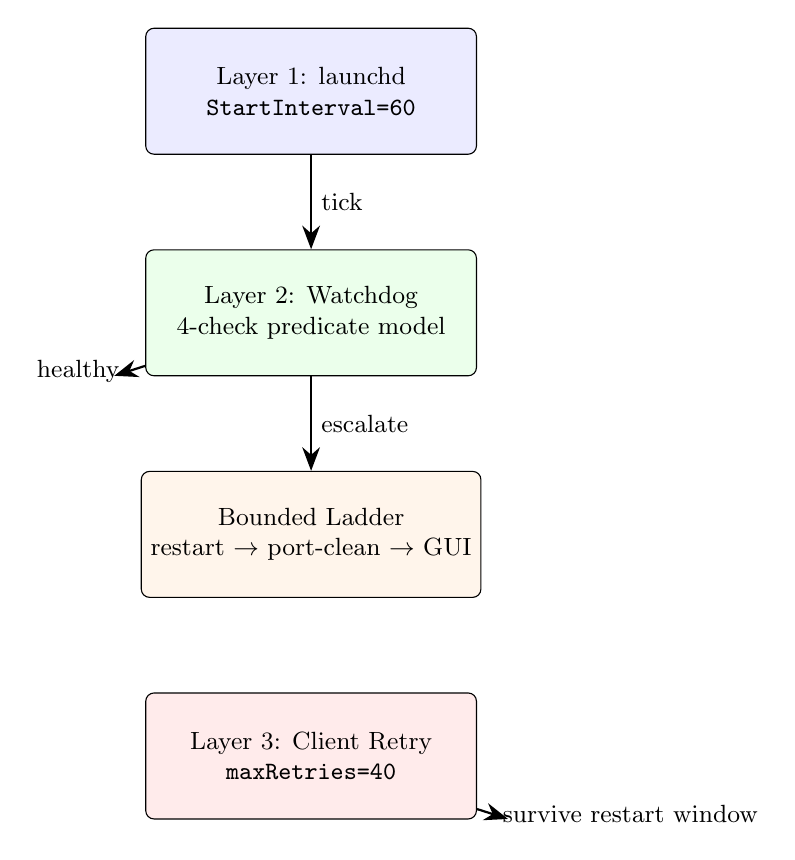
\begin{tikzpicture}[
  box/.style={draw, rounded corners=3pt, minimum width=4.2cm, minimum height=1.6cm,
              align=center, font=\small},
  arrow/.style={-{Stealth[length=3mm]}, thick}
]
\node[box, fill=blue!8] (launchd) {Layer 1: launchd\\ \texttt{StartInterval=60}};
\node[box, fill=green!8, below=1.2cm of launchd] (watchdog) {Layer 2: Watchdog\\ 4-check predicate model};
\node[box, fill=orange!8, below=1.2cm of watchdog] (ladder) {Bounded Ladder\\ restart $\to$ port-clean $\to$ GUI};
\node[box, fill=red!8, below=1.2cm of ladder] (client) {Layer 3: Client Retry\\ \texttt{maxRetries=40}};

\draw[arrow] (launchd) -- node[right, font=\small]{tick} (watchdog);
\draw[arrow] (watchdog) -- node[right, font=\small]{escalate} (ladder);
\draw[arrow] (watchdog) -- node[left, font=\small]{healthy} ++(-2.5,-0.8);

\draw[<->, arrow] (client) -- node[right, font=\small]{survive restart window} ++(2.5,-0.8);
\end{tikzpicture}
\caption{Three-layer defense: launchd tick $\to$ watchdog predicate evaluation $\to$ bounded escalation ladder, with client-side retry budget spanning the restart window.}
\label{fig:arch}
\end{figure}

% ═══════════════════════════════════════════════════════════════════
\section{Failure Taxonomy}\label{sec:taxonomy}

Table~\ref{tab:fails} lists the six classes with their production incidence. Figure~\ref{fig:taxonomy} shows the causal relationships between failure classes and the recovery actions that address them.

\begin{table}[t]\centering
\small
\renewcommand{\arraystretch}{1.3}
\begin{tabular}{@{}lll@{}}
\toprule
Class & Mechanism & Incidence (13d) \\
\midrule
F1 Engine wedge   & Metal layer stuck; requests accepted, no tokens & 2 episodes (Sep 8) \\
F2 Port squatter  & Stale listener on :8000 after restart; retry spin & 26 port-cleans \\
F3 SIGKILL/OOM    & System kill; launchd does not auto-relaunch GUI app & 96 fallbacks \\
F4 Stale registry & \texttt{loaded\_models} out of sync after model switch & 79 recoveries (v5 era) \\
F5 Prefill guard rejection & Predictable HTTP 400 at memory ceiling (by design) & n/a \\
F6 Client retry amplification & \texttt{mode:always} retries $\times$ restart window = death loop (pre-fix) & 1 episode \\
\bottomrule
\end{tabular}
\caption{Failure classes and production incidence (Sep 27 -- Sep 9, 18{,}516 ticks). F4 dominates the v5 era and was eliminated by the empty-registry-aware Check B in v6.}
\label{tab:fails}
\end{table}

\begin{figure}[t]\centering
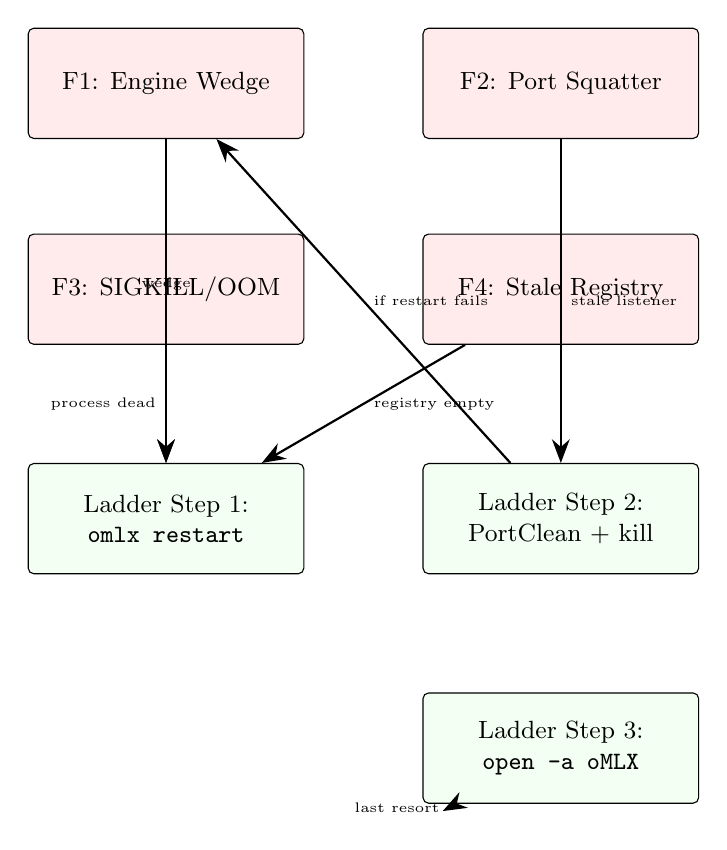
\begin{tikzpicture}[
  fbox/.style={draw, rounded corners=2pt, minimum width=3.5cm, minimum height=1.4cm,
               align=center, font=\small},
  rbox/.style={draw, rounded corners=2pt, minimum width=3.5cm, minimum height=1.4cm,
               align=center, font=\small, fill=green!5},
  arrow/.style={-{Stealth[length=3mm]}, thick}
]
\node[fbox, fill=red!8] (F1) {F1: Engine Wedge};
\node[fbox, fill=red!8, right=1.5cm of F1] (F2) {F2: Port Squatter};
\node[fbox, fill=red!8, below=1.2cm of F1] (F3) {F3: SIGKILL/OOM};
\node[fbox, fill=red!8, right=1.5cm of F3] (F4) {F4: Stale Registry};

\node[rbox, below=1.5cm of F3] (R1) {Ladder Step 1:\\ \texttt{omlx restart}};
\node[rbox, right=1.5cm of R1] (R2) {Ladder Step 2:\\ PortClean + kill};
\node[rbox, below=1.5cm of R2] (R3) {Ladder Step 3:\\ \texttt{open -a oMLX}};

\draw[arrow] (F1) -- node[above, font=\tiny]{wedge} (R1);
\draw[arrow] (F2) -- node[right, font=\tiny]{stale listener} (R2);
\draw[arrow] (F3) -- node[left, font=\tiny]{process dead} (R1);
\draw[arrow] (F4) -- node[right, font=\tiny]{registry empty} (R1);
\draw[arrow] (R2) -- node[right, font=\tiny]{if restart fails} (F1);
\draw[arrow] (R3) -- node[left, font=\tiny]{last resort} ++(-1.5,-0.8);
\end{tikzpicture}
\caption{Causal mapping from failure classes to recovery ladder steps. F2 (port squatter) is the only class that requires Step 2; all others are resolved by Step 1 or eliminated by versioned fixes.}
\label{fig:taxonomy}
\end{figure}

The F1/F3 distinction matters: \texttt{oMLX restart} fixes wedges but a squatted port makes the restart itself fail, creating the F2 spin that motivated listener-only cleanup.

% ═══════════════════════════════════════════════════════════════════
\section{Detection: A Self-Interference-Free Health Model}\label{sec:detection}

A watchdog tick $t$ evaluates four predicates on the server state:
\begin{align}
A(t) &: \texttt{/api/status reachable within 5s} \\[0.3em]
B(t) &: \big(\texttt{loaded\_models} = \varset\big) \lor \big(\exists m{:}\; m.\texttt{registered}\big) \\[0.3em]
C(t) &: \neg\,\textsf{busy}(t) \;\lor\; \textsc{IdleProbe}(\texttt{max\_tokens}=4) = \textsc{ok} \\[0.3em]
D(t) &: \neg\,\big(\textsf{workInFlight}(t) \land \Delta t_{\text{token}}(t) \ge 900\,\text{s}\big)
\end{align}

where $\textsf{busy}(t)$ is \emph{provably} the server's own queue counter (\texttt{active+waiting}$>$0). The health predicate is $H(t)=A\land B\land C\land D$.

\noindent\textbf{Self-interference-freedom.} Check C fires \emph{only when the queue is provably empty}; a long decode (hours of tool-calling) keeps \texttt{active}$\ge 1$ and is never probed. Check D requires work \emph{in flight} with a frozen token counter -- idle servers have no reference to freeze. The v2 design (log mtime) violated this: cancelled requests wrote log lines, marking dead engines ``busy''.

\noindent\textbf{Empty-registry awareness (F4 fix).} After a model switch the registry may transiently be empty; $B(t)$ treats $\varset$ as healthy rather than triggering a restart storm (79 such events in the v5 era).

Figure~\ref{fig:detection} shows the decision flow for a single tick.

\begin{figure}[t]\centering
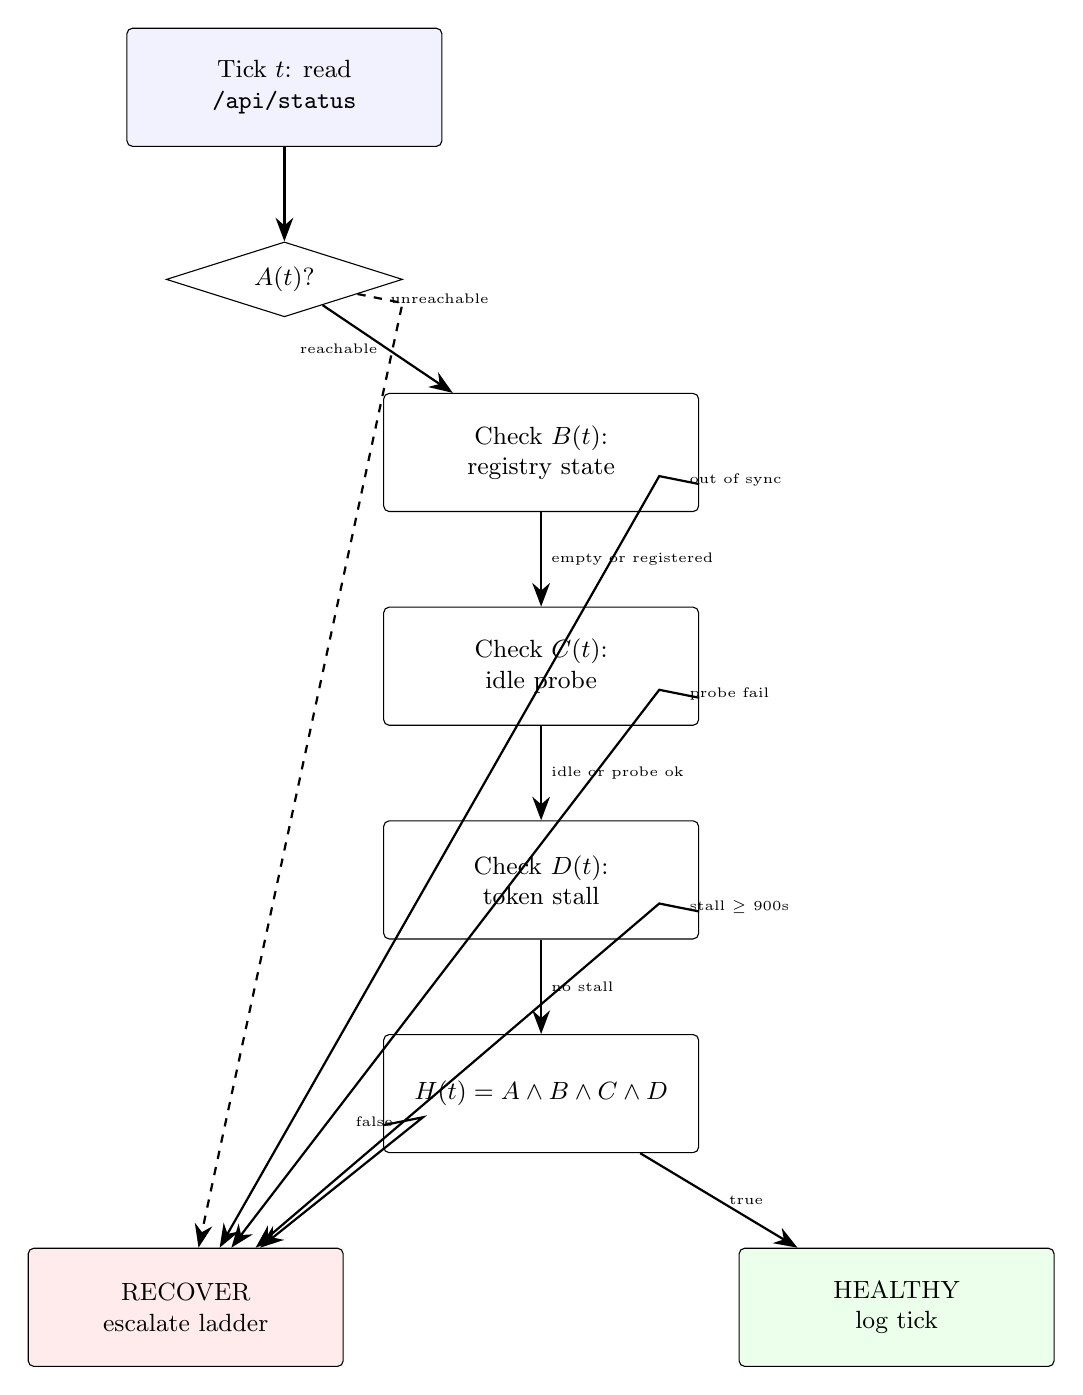
\begin{tikzpicture}[
  dbox/.style={draw, rounded corners=2pt, minimum width=4cm, minimum height=1.5cm,
               align=center, font=\small},
  ddec/.style={draw, diamond, aspect=2.5, minimum width=3cm, align=center, font=\small},
  arrow/.style={-{Stealth[length=3mm]}, thick}
]
\node[dbox, fill=blue!5] (start) {Tick $t$: read\\ \texttt{/api/status}};
\node[ddec, below=1.2cm of start] (A) {$A(t)$?};
\node[dbox, below right=1.2cm and 0.5cm of A] (B) {Check $B(t)$:\\ registry state};
\node[dbox, below=1.2cm of B] (C) {Check $C(t)$:\\ idle probe};
\node[dbox, below=1.2cm of C] (D) {Check $D(t)$:\\ token stall};
\node[dbox, below=1.2cm of D] (H) {$H(t)=A\land B\land C\land D$};
\node[dbox, below right=1.2cm and 0.5cm of H, fill=green!8] (ok) {HEALTHY\\ log tick};
\node[dbox, below left=1.2cm and 0.5cm of H, fill=red!8] (recover) {RECOVER\\ escalate ladder};

\draw[arrow] (start) -- (A);
\draw[arrow, dashed] (A) -- node[right, font=\tiny]{unreachable} ++(1.5,-0.3) -- (recover);
\draw[arrow] (A) -- node[left, font=\tiny]{reachable} (B);
\draw[arrow] (B) -- node[right, font=\tiny]{empty or registered} (C);
\draw[arrow] (B) -- node[right, font=\tiny]{out of sync} ++(1.5,-0.3) -- (recover);
\draw[arrow] (C) -- node[right, font=\tiny]{idle or probe ok} (D);
\draw[arrow] (C) -- node[right, font=\tiny]{probe fail} ++(1.5,-0.3) -- (recover);
\draw[arrow] (D) -- node[right, font=\tiny]{no stall} (H);
\draw[arrow] (D) -- node[right, font=\tiny]{stall $\ge$ 900s} ++(1.5,-0.3) -- (recover);
\draw[arrow] (H) -- node[right, font=\tiny]{true} (ok);
\draw[arrow] (H) -- node[left, font=\tiny]{false} ++(-1.5,-0.3) -- (recover);
\end{tikzpicture}
\caption{Decision flow for a single watchdog tick. Each check is evaluated only if all prior checks pass; any failure routes to the bounded escalation ladder (Sec.~\ref{sec:recovery}).}
\label{fig:detection}
\end{figure}

% ═══════════════════════════════════════════════════════════════════
\section{Recovery: A Bounded Escalation Ladder}\label{sec:recovery}

On $H(t)=\textsc{false}$, the watchdog escalates:
\begin{enumerate}[nosep]
  \item $\texttt{omlx restart --timeout 240}$ (engine-level, no process kill)
  \item On failure: \textsc{PortClean} -- identify the PID with $\texttt{lsof -sTCP:LISTEN}$ on :8000, \texttt{kill}, 30\,s grace, then \texttt{kill -9}; retry step~1
  \item Last resort: $\texttt{open -a oMLX}$ (GUI relaunch)
\end{enumerate}

A PID lockfile prevents re-entrant ticks. \textbf{Safety of PortClean:} the kill target is verified as the sole TCP listener on port 8000 -- never a process list match -- so no unrelated process can be signaled. The ladder is bounded: at most one restart, one port-clean, one GUI launch per tick; the next tick re-evaluates from a clean state.

Figure~\ref{fig:ladder} shows the ladder with timing bounds.

\begin{figure}[t]\centering
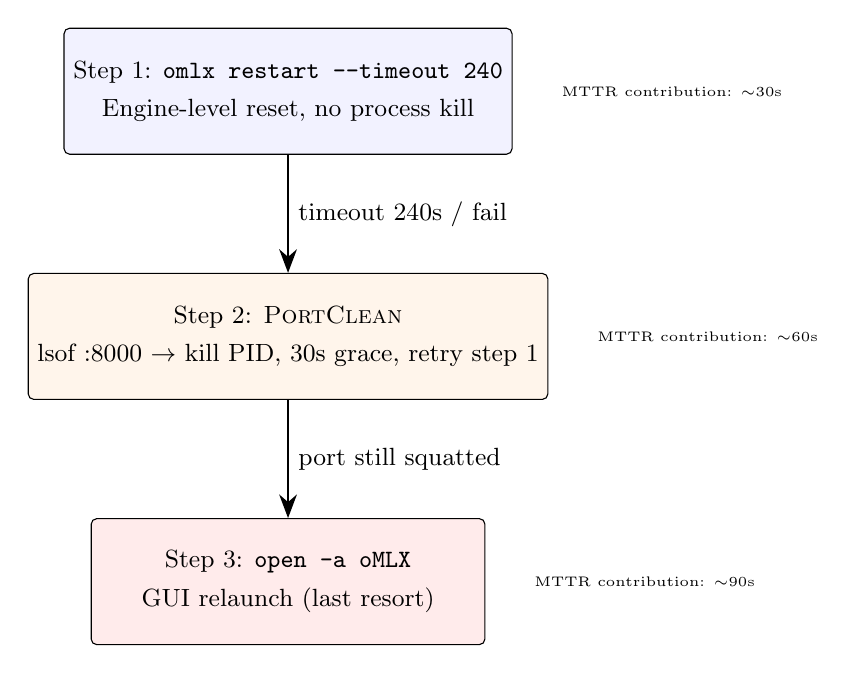
\begin{tikzpicture}[
  lbox/.style={draw, rounded corners=2pt, minimum width=5cm, minimum height=1.6cm,
               align=center, font=\small},
  arrow/.style={-{Stealth[length=3mm]}, thick}
]
\node[lbox, fill=blue!5] (step1) {Step 1: \texttt{omlx restart --timeout 240}\\[0.3em]
  {\small Engine-level reset, no process kill}};
\node[lbox, fill=orange!8, below=1.5cm of step1] (step2) {Step 2: \textsc{PortClean}\\[0.3em]
  {\small lsof :8000 $\to$ kill PID, 30s grace, retry step 1}};
\node[lbox, fill=red!8, below=1.5cm of step2] (step3) {Step 3: \texttt{open -a oMLX}\\[0.3em]
  {\small GUI relaunch (last resort)}};

\draw[arrow] (step1) -- node[right, font=\small]{timeout 240s / fail} (step2);
\draw[arrow] (step2) -- node[right, font=\small]{port still squatted} (step3);

\node[font=\tiny, right=0.5cm of step1] {MTTR contribution: $\sim$30s};
\node[font=\tiny, right=0.5cm of step2] {MTTR contribution: $\sim$60s};
\node[font=\tiny, right=0.5cm of step3] {MTTR contribution: $\sim$90s};
\end{tikzpicture}
\caption{Bounded escalation ladder with timing bounds. Each step is attempted at most once per tick; the next tick re-evaluates from a clean state.}
\label{fig:ladder}
\end{figure}

% ═══════════════════════════════════════════════════════════════════
\section{Evaluation: 13 Days in Production}\label{sec:eval}

\noindent\textbf{Setup.} Apple M5 Max, 128\,GB unified memory; macOS Tahoe; oMLX v0.6.x serving Qwen3.8-27B (oQ8e, later oQ4e) with MTP; launchd \texttt{StartInterval=60}. Clients: DSH Web GUI, OpenClaw/Hermes gateways via the same endpoint.

\begin{table}[t]\centering
\small
\renewcommand{\arraystretch}{1.3}
\begin{tabular}{@{}lrr@{}}
\toprule
Metric & Value \\
\midrule
Total ticks / wall time          & 18{,}516 / 13.2 days \\
HEALTHY idle ticks               & 13{,}527 (73.0\%) \\
BUSY ticks                       & 4{,}188 (22.6\%) \\
Recovery events completed        & 79 RECOVERED, 0 STILL\_DOWN after ladder \\
Mean time to detect (MTTD)       & $\le 60$\,s (one tick) \\
Mean time to recover (MTTR)      & $<$ 4\,min (restart + reload observed) \\
False-positive restarts (v6 era) & 0 in the final 48\,h window \\
Decode throughput (BUSY ticks)   & median 1.9 tok/s; p90 7.6 tok/s (long-context, TQKV+MTP) \\
\bottomrule
\end{tabular}
\caption{Production statistics, \texttt{watchdog.log}, 2026-08-27 $\rightarrow$ 2026-09-09.}
\label{tab:eval}
\end{table}

The Sep 8 window (F1 wedge + F4 stale registry, pre-v6) shows the ladder under load: 96 fallback escalations with all recoveries completed, and the v4 port-clean fix eliminating the F2 spin. Post-v6 (Sep 9), zero false-positive restarts in 48\,h.

\noindent\textbf{Throughput context.} With oQ4e + MTP (accept rate 85--96\%) + TurboQuant Q4 KV cache, short-context decode reaches $\sim$30--50 tok/s; long-context (80k+ tokens) settles at 12--25 tok/s, consistent with the M5 Max $\sim$614\,GB/s memory-bandwidth bound on weight+KV reads. Availability (this paper) and throughput are orthogonal: the three-layer defense multiplies them.

Figure~\ref{fig:timeline} shows the event timeline across the 13-day trace.

\begin{figure}[t]\centering
\begin{tikzpicture}[xscale=0.35, yscale=1]
\draw[->] (0,-0.5) -- (26,0) node[right]{days};
\draw[->] (-0.5,-12) -- (0,1) node[left]{events};

% Day 0-5: healthy
\draw[blue, thick] (1,-2) -- (4.5,-2);
\node[font=\tiny, above] at (2.75,-2) {HEALTHY};

% Day 6-8: F1 + F4 window
\draw[red, thick] (5,-2) -- (8.5,-2);
\node[font=\tiny, above] at (6.75,-2) {F1 wedge + F4};
\node[font=\tiny, below] at (6.75,-2) {96 fallbacks};

% Day 8: v4 port-clean fix
\draw[orange, thick] (8.5,-2) -- (9,-2);
\node[font=\tiny, above] at (8.75,-2) {v4 fix};

% Day 9-13: v6 era, healthy
\draw[green!60!black, thick] (9,-2) -- (13.5,-2);
\node[font=\tiny, above] at (11.25,-2) {v6: 0 false positives};

% Tick marks
\foreach \x/\lbl in {1/Day 0, 3.5/Day 4, 7/Day 8, 10.5/Day 12}
  \draw (\x,-0.3) -- (\x,0) node[below, font=\tiny]{\lbl};

% Event counts
\node[font=\small] at (6.75,0.8) {13{,}527 HEALTHY};
\node[font=\small] at (11.25,0.8) {4{,}188 BUSY};
\end{tikzpicture}
\caption{Event timeline across the 13-day trace. The Sep 8 window (F1+F4) shows the ladder under load; post-v6, zero false-positive restarts.}
\label{fig:timeline}
\end{figure}

% ═══════════════════════════════════════════════════════════════════
\section{Related Work}\label{sec:related}

Kubernetes liveness/readiness probes assume an orchestrator with process-kill authority; our ladder is the single-host analog where the ``orchestrator'' (launchd) deliberately does \emph{not} auto-relaunch a GUI app. SRE self-healing patterns (bounded escalation, no retry amplification) map directly onto ladder steps 1--3 and the client-side \texttt{maxRetries=40} bound. Local-LLM tooling (Ollama, llama.cpp server) ships no equivalent watchdog; DFlash/MTP speculative decoding improves per-request throughput but does not address partial availability.

% ═══════════════════════════════════════════════════════════════════
\section{Threats to Validity}

Single operator, single machine, one server version family. The \texttt{loaded\_models} field is a stable API surface but not contractual; Check B degrades gracefully (empty-aware) if renamed. Throughput figures are trace-derived medians, not controlled benchmarks.

% ═══════════════════════════════════════════════════════════════════
\section{Conclusion}

A 180-line shell script with four non-conflicting predicates and a bounded ladder provides full self-healing for an unorchestrated local LLM server: MTTD $\le 60$\,s, MTTR $<$4\,min, zero human interventions across 13 days of agent workloads. The design generalizes to any OpenAI-compatible local backend (llama.cpp, Ollama) by substituting the restart primitive.

% ═══════════════════════════════════════════════════════════════════
\section*{Artifact Availability}

Watchdog + installer: \url{https://github.com/ricky8848/omlx-watchdog} (MIT, v6.1; \texttt{curl | bash}). Three-layer config: \url{https://github.com/ricky8848/mac-m5-128g-omlx-settings}. Full de-identified trace: \texttt{docs/paper/production-data.json} in the artifact repository.

\end{document}
